\clearpage

\section*{数学と物理の関係}
物理と数学は高校までは別物として授業を行っているが、ちゃんと物理をしていくと物理と数学の違いがわからなくなるくらいに物理では数学をよく使っている。私が思うに数学は自然現象を記述していくための言語である。自然現象自体にもともと名前がついているわけはないし取扱説明書があるわけはない。でも人間は自然現象を理解していくためには言語化しないといけない。だけども日本語とか英語とかで自然現象を記述するのは難しいしきっと莫大な量になってしまう。そこで登場してくるのが数学である。数学を使用するととても簡単に記述することができてしまうし数学はどの国に行っても記述の方法は一緒なので翻訳する必要はない。といったことで物理では数学は必須言語なのである。
\section*{この文の構成}
本当はもう少し簡単なところから書いていこうかとも思ったのですが、時間などの関係上その部分はなくなってしまいました。そのため簡単な数学や力学をかじってないと結構専門的な文章になっていると思うので物理をまったくやってない人は共鳴というものを説明するにはこんなにも数学を使うんだなあと思うくらいで目を通してくださると幸いです。



\newpage

\chapter{強制振動~共鳴まで}
\section{減衰振動}
今回は共鳴というものを数式的にどのようにわかるかということを示してみる。\\
まず、抵抗力の働いたばねの振動を考える。この振動の運動の運動方程式は、
\begin{eqnarray}
m\frac{d^2x}{dt^2}+b \frac{dx}{dt} + kx&=&0 \\
\frac{d^2x}{dt^2}+2\gamma \frac{dx}{dt} + {\omega_0}^2 x&=&0\\
\left(\gamma = \frac{b}{2m} ,  {\omega_0}^2  = \frac{k}{m} \right) \nonumber
\end{eqnarray}

で表すことができる。この微分方程式は二階の同次線形微分方程式である。この微分方程式の一般解を求める。$x=e^{\lambda t}$とおいて式(2)に代入すると、
\begin{eqnarray}
{\lambda}^2+2\gamma \lambda+{\omega_0}^2 = 0 \nonumber \\
\lambda = -\gamma \pm \sqrt{{\gamma}^2-{\omega_0}^2}
\end{eqnarray}
となる。よってこの$\lambda$の解は三つの場合に分けることができる。場合分けを行って式(2)の一般解を求める。\\
(1)$\omega_0 < \gamma$つまり復元力よりも抵抗力が大きい時を考える。この条件では$\lambda$が実数値を持つよって式(2)解の重ね合わせで表現できるので
\begin{eqnarray}
x(t)&=&C_1e^{-\gamma t}e^{\sqrt{{\gamma}^2-{\omega_0}^2}t}+C_2e^{-\gamma t}e^{-\sqrt{{\gamma}^2-{\omega_0}^2}t}
\end{eqnarray}
という形で表される。この式の振幅はすぐに減衰してしまい振動しない(過減衰)\\
\begin{figure}[H]
\centering
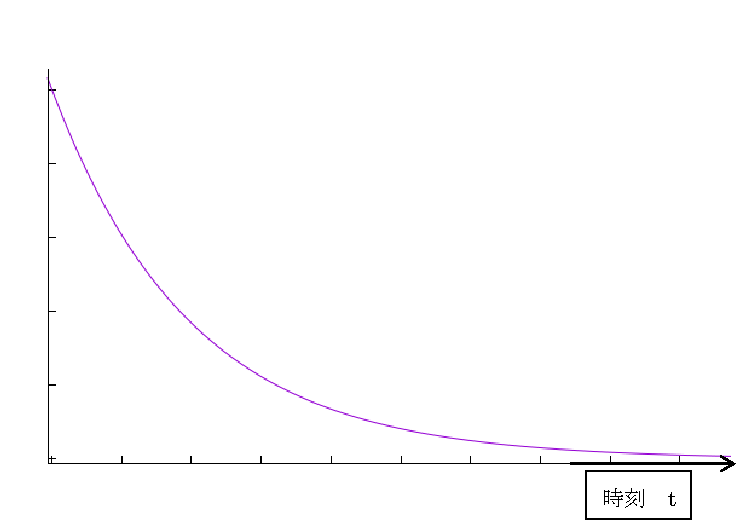
\includegraphics[height=7cm,clip]{kadono/image/gensui.pdf}
\label{fig:ele1}
\caption{過減衰}
\end{figure}
(2)$\omega_0 = \gamma$つまり$\lambda$が重根を持つとき、解が一つしか持たない、よって変数変化法を用いてこの場合の一般解を求めると、
\begin{eqnarray}
x(t)&=(At+B)e^{-\gamma t}
\end{eqnarray}
となる。この場合も同じように指数関数的に減衰する。(臨界減衰)\\
(3)$\omega_0 > \gamma$つまり抵抗力が小さい時を考える。この条件では$\lambda$が虚数となる。よって式(3)の$\lambda$の解を書き換えると
\[
\lambda = \pm i\omega - \gamma  \ \ \ \ \ \ \  (\omega= \sqrt{\omega^2-\gamma^2})
\]
とすると、(1)と同じように表すことができる。
\begin{eqnarray}
x(t)	&=&C_1e^{-\gamma t}e^{-i\omega t}+C_2e^{-\gamma t}e^{+i\omega t} \nonumber\\
	&=&e^{-\gamma t}(C_1e^{-i\omega t}+C_2e^{+i\omega t})\nonumber\\
	&=&Ce^{-\gamma t}\cos (\omega t +\phi)
\end{eqnarray}
となる。この振動は単振動のような振動しながら振幅は指数関数的に徐々に減少していく。(減衰振動)
\begin{figure}[H]
\centering
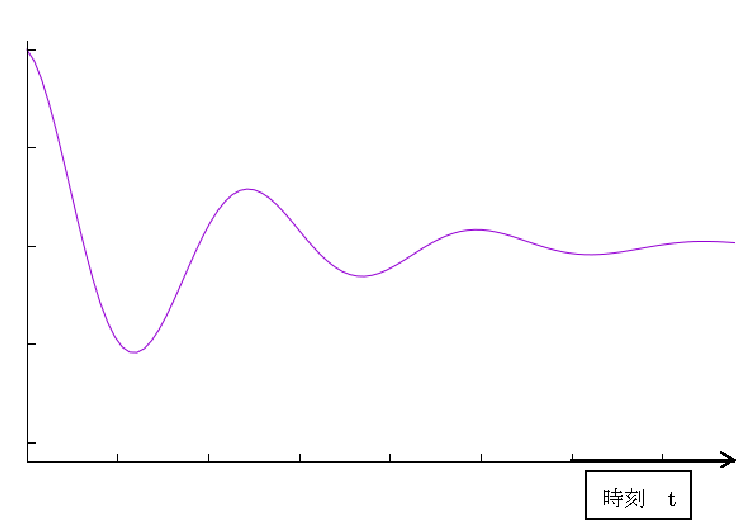
\includegraphics[height=7cm,clip]{kadono/image/gensui1.pdf}
\label{fig:ele1}
\caption{減衰振動}
\end{figure}


\section{強制振動}
強制振動とは、外部から周期的に力を加えられることによって振動する振動を強制振動という。式(1)に外部からの力の項を加えると
\begin{eqnarray}
m\frac{d^2x}{dt^2}+b \frac{dx}{dt} + kx&=& F(t)
\end{eqnarray}
となる。ここで$F(t)=F_0\cos {\omega t}$という形の微分方程式を考える。

\begin{eqnarray}
\frac{d^2x}{dt^2}+2\gamma \frac{dx}{dt} + {\omega_0}^2 x&=&f\cos{\omega t}\ \ \ \ \ (f = F_0/m)
\end{eqnarray}
となる。この微分方程式は非同次微分方程式である。このような微分方程式の一般解は同次の一般解と非同次の特解の和で求められることが知られている。なぜかは数学の得意な人に聞いて下さい。\\
同次の一般解はもう求めてあるので、必要なのは(8)の特解である。しかしなかなかこの微分方程式は求まらないので虚数の項を加えてみたらうまくいくらしいので、そうしてみる。よって(8)の右辺に
\[
if\sin{\omega t}
\]
を加えてみるそうすると
\begin{eqnarray}
\frac{d^2x}{dt^2}+2\gamma \frac{dx}{dt} + {\omega_0}^2 x&=&fe^{i\omega t}
\end{eqnarray}
となる。これだとうまくいきそうなのでこれをこれで特解を求めてみることにする。まず特解を
\begin{eqnarray}
x_s = Ae^{i\omega t}
\end{eqnarray}
と仮定して(9)に入れてみると....
\begin{eqnarray}
(-\omega^2 +2\gamma \omega i + {\omega_0}^2)Ae^{i\omega t}=fe^{i\omega t}
\end{eqnarray}
となりこれを$A$について解くと、
\begin{eqnarray}
A=\frac{f}{\sqrt{({\omega_0}^2-\omega^2)^2+4\gamma^2\omega^2}}e^{i\psi}
\end{eqnarray}
となる。これで(9)の特解を求めることができる。
\begin{eqnarray}
x_s = \frac{f}{\sqrt{({\omega_0}^2-\omega^2)^2+4\gamma^2\omega^2}}e^{i\omega t +\psi}
\end{eqnarray}
となる。でも私たちが知りたいのは(8)の特解である。これは、(13)の実数部分がそのものである。なぜそうなるかは考えてみると結構早くわかるが、簡単に言うと複素数を微分するとき、実数部分の微分に虚数の部分の微分がかかわってくることがないからである。\\
よって、式(8)の特解は
\begin{eqnarray}
x_s = \frac{f}{\sqrt{({\omega_0}^2-\omega^2)^2+4\gamma^2\omega^2}}\cos(\omega t +\psi)
\label{eq:tokkai}
\end{eqnarray}
よって求まった!
\section{ここから何が分かるのか}
ようやく強制振動の運動方程式の一般解が求まったですが、そもそもここから何が読み取れるのか何が分かるのかをわからないと意味がない、\\
前の部分では、正直言うと強制振動の特解しか求めていない、これには理由が存在している。それは、非斉次の微分方程式の特解は斉次の一般解と特解との和で表せる。という話であった。ここで斉次の一般解とはそもそも減衰していってしまうものであり、それはいつかなくなってしまう項である。そんな未来性のない項を考えても仕方がないというのでじゃあ特解だけでいいやということで特解だけをあえて残した。\\
特解(\ref{eq:tokkai})の式は基本の形は単振動の式である。外力で変えられるものは
\[
f , \omega
\]
である。でも$f$を変えてもただ単調に増えていくだけでそこまで特徴を見出せない。では$\omega$はを変えていくとどのように変化していくのかを考えてみるとある特徴的な現象を説明することができる。まずは特解(\ref{eq:tokkai})の式の形について考えてみる。この特解の形を簡単に記号に置き換えて考えてみると
\begin{eqnarray}
  x_s = A\cos(\omega t + \psi)  \left(A = \frac{f}{\sqrt{({\omega_0}^2-\omega^2)^2+4\gamma^2\omega^2}} \right)
\end{eqnarray}
という形であることが分かる。この形は単振動の式とまったく変わらない。$A$は本当にただの振幅なのかどうかが気になるひとがいるだろう。しかしただの振幅である。$A$で使ってる変数は$\omega_0\ \omega \ \gamma \  f$である。一つ一つ見ていくと$\omega_0$は減衰振動の振動数であるので時間に依存しない変数である。$\gamma$は上で定数として定義していたので時間によって変化されてしまったら困る。$\omega ,\ f$は前で述べたように外力の振動数のその大きさであるのでこれも時間に依存してしまったらとても難しい運動になってしまうのでひとまず時間に依存しない変数とする。\\
以上より、ここで特解は上の式で表すことができることが分かった。ここでようやく$\omega$を変えることによってどんな面白いことがあるかを考えて見ることにします。$\omega$を変えると特解のどこが変化するかというと上の式の$A$であるつまり単振動の振幅の値である。振幅の値が変化するということはその振動が大きくなるということである。振幅が大きくなるとその運動を人間が見やすくなるということである。そのほかにも波のエネルギーは振幅の二乗で求めることができることが知られていてつまり振幅が大きくなるとその波のエネルギーは大きくなっていく。このエネルギーの源は何だったかを考えると、外力である。特解の振幅が大きいほど外力のエネルギーを効率よく波が吸収しているということである。この現象を共鳴という。\\
$\omega$がどのようになったら振幅の値が大きくなるのかを考える。$A$が最大になるためには$A$の分母が最小になるときなのでその時は$\omega = \omega_0$の時である。ここで$\gamma<\omega_0$であることに注意すると簡単に求めることができる。\\
この$\omega$計算的にもとめることはここでできた。しかし、実際はこの$\omega$を実験で求める必要がある。ここで$Aを\omega$の関数としてグラフを作成してみると下図のようになる。
\begin{figure}[H]
\centering
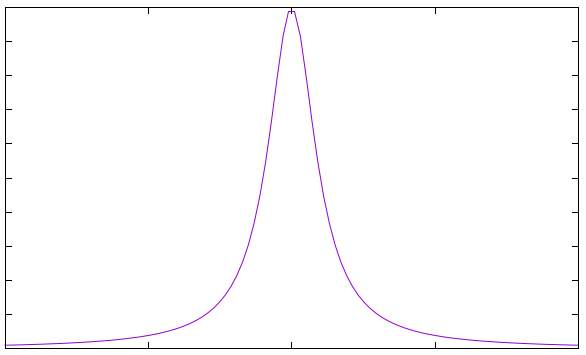
\includegraphics[height=7cm,clip]{kadono/image/reso.png}
\label{fig:reso}
\caption{共鳴曲線}
\end{figure}

\newpage

\chapter{共鳴現象を利用した実験例}
ここまで共鳴現象というものを理論的に数学的に記述してきた。この現象がいったいどのくらい物理の実験や現実世界で使われいるのかの一例をここから書いていきたいと思います。\\
ここから書いてあるものは実際に私が実験したものを抜粋してきたものになっています。概要を見たら大体実験の内容が分かるかと思いますが、簡潔に言うとLC回路が共鳴するときの振動数を図ってコイルの自己インダクタンスを求めようということです。
\begin{center}
\section*{LC回路を使用した自己インダクタンスの測定}
\end{center}
\subsection*{概要}
ICカードに使われている電気回路に注目して実験を行った。ICカードの中にはLC直列回路が入っておりその回路が共鳴現象を起こすことによって電力が供給されている。今回の実験はこのICカードに利用されている電気回路をなるべく再現しLC直列回路に共鳴現象が起きることを確認しその実験のデータからコイルの自己インダクタンスを求めた。結果として今回作製したコイルの自己インダクタンスは$7.5\times 10^{-5}\ {\rm H}$であることが分かった。


\section{序論}
今日では従来必需品であったものがどんどんなくなってきている。その中の一つは現金である。今では電車に乗るときはICOKAやSUIKAなどのICカードを使用しいる。ICカードは今やいろんなところで使用されているが、このカードの特徴は機器にかざすだけで商品の支払いが終わる。カードと機器の間はもちろんだがつながってはいない、加えてカードのほうには電力原が存在していない。どうしてこんなただカードで情報のやり取りができるのか、どうして電力原がないカードに電流が通るのかこの疑問について考えていきたいと思う。ICカードには電気回路が入っている。この回路簡単に言うとLC直列回路である。この中には電源がないのにこの回路が動作するのかを説明するのにLCR直列回路の共鳴現象について説明たいと思う。いま考えるLCR直列回路は図\ref{fig:ele}の(A)に示す。この回路で時刻をt、コイルの自己インダクタンスをL、抵抗をR、コンデンサの電気容量をC、交流電圧を$V_0 \cos{\omega t}$、回路の中を流れる電流を$i$とするとこの電気回路の微分方程式を次に示す。
\begin{eqnarray}
L\frac{d^2i}{dt^2}+R\frac{di}{dt}+\frac{i}{C}=V_0\cos{\omega t}
\end{eqnarray}
この式の特解は
\begin{eqnarray}
i=I\sin(\omega t + \phi)\ \ \ \ \ \left(I=\frac{V_0}{\sqrt{R^2+(\omega L- \frac{1}{\omega C})^2}}\right)
\end{eqnarray}
となる。ここで振幅が最大になるような$\omega $は$I$の分母の値が最小になるときなので
\begin{eqnarray}
\omega =\omega_0=\frac{1}{\sqrt{LC}}=\frac{1}{\sqrt{L}}C^\frac{1}{2}
\end{eqnarray}
となる。\\
以上よりLCR直列回路にある特定の周波数の電圧を加えると電流の値が最大の値をとることが分かった。この関係をグラフにすると図\ref{fig:ele}の(B)のようになる。ここで
\[
Q=\frac{\omega_0}{\omega_2-\omega_1}
\]
と定義されている共鳴の鋭さというものがある。$\omega_1,\omega_2$はそれぞれ$V_m/\sqrt{2}$の値をとるときの各振動数である。このQ値というのは図\ref{fig:ele}の(C)の共鳴振動数の周辺の鋭さを示す物である。このQ値が示す物理的な意味はどれだけエネルギーを安定的に吸収したかを表すものである。

以上で電気回路の共鳴現象については理論的には分かった。ここでICカードには電力源がないのにどのように電力を供給しているのかを考える。コイルは時間的に磁場が変化する空間に置かれるとあるその磁場の変化に対応した電圧が生じる。この現象は発電システムにも利用されている。この現象を利用してICカードに電力が供給されている。この現象を利用した共鳴回路を図\ref{fig:ele}の(C)に示す。今回の実験はこの現象を利用しLC直列回路に電力を供給し共鳴現象を起こした。\\
数式(3)からわかるように固有角振動数は電気容量の-1/2倍に比例することが分かる。今回の実験はコイルの自己インダクタンスを求めることを目的とし固有振動数と電気容量の間の関係を調べた。
\\
\begin{figure}[H]
\centering
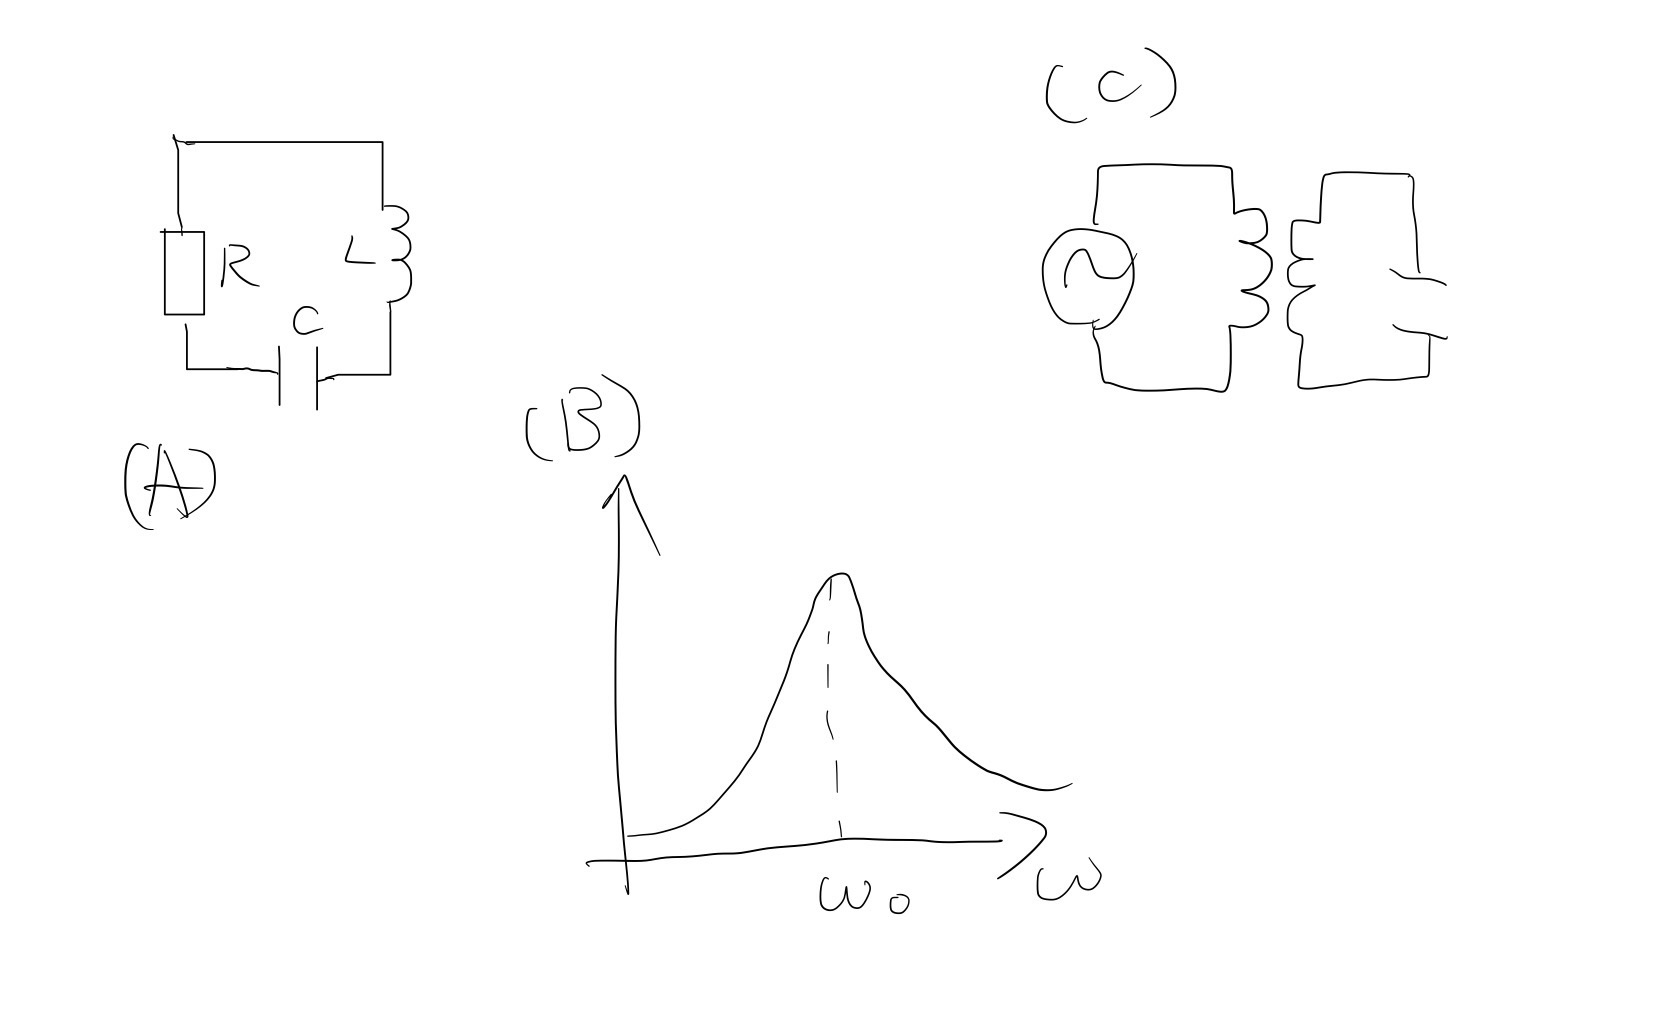
\includegraphics[height=8cm,clip]{kadono/image/houhou.jpg}
\label{fig:ele}
\caption{(A):LCR直列回路、(B)振動数と振幅との関係のグラフ、(C):コイルを使用して電力を供給したLC直列回路}
\end{figure}
\newpage
 \section{実験方法}
今回行った実験の模式図を図\ref{fig:ele1}に示す。回路図上のコイル部分はアクリル製のパイプ(外形21 mm内径18 mm)に0.4 mmの被覆銅線を使用した。一次コイル(ファンクションジェネレーターにつながっている方)に30回巻き、二次コイル(コンデンサにつながっている方)を90回巻きにして一次コイルと二次コイルは同じパイプ上に間を開けて巻いた。(このときコイルに巻いた銅線のはじめと終わりをやすりなどでこすり表面の被覆を落とし電流が通るようにする)\\
 コンデンサを図のようにつなげファンクションジェネレータによって一次コイルにかかる振動数を変えて振幅の値が最大になる振動数(共鳴振動数)を探した。見つけた共鳴振動数の$\pm 0.1$MHzの範囲で$0.01$MHz刻みでオシロスコープから振幅の値を読みとった。共鳴振動数での周辺で振動数と振幅のデータが20個を得られた。このデータを使用して横軸に振動数、縦軸に振幅をとったグラフ(共鳴曲線)を書き、このデータから共鳴の鋭さ(Q値)を求めた。コンデンサの電気容量を変化させて再度共鳴振動数での周辺の振動数と振幅のデータをとりそのデータからQ値を求めた。各電気容量での共鳴振動数を求めたのち電気容量と共鳴振動数の関係のグラフを書きそのグラフから今回使用した自己インダクタンスを求めた。

\begin{figure}[H]
\centering
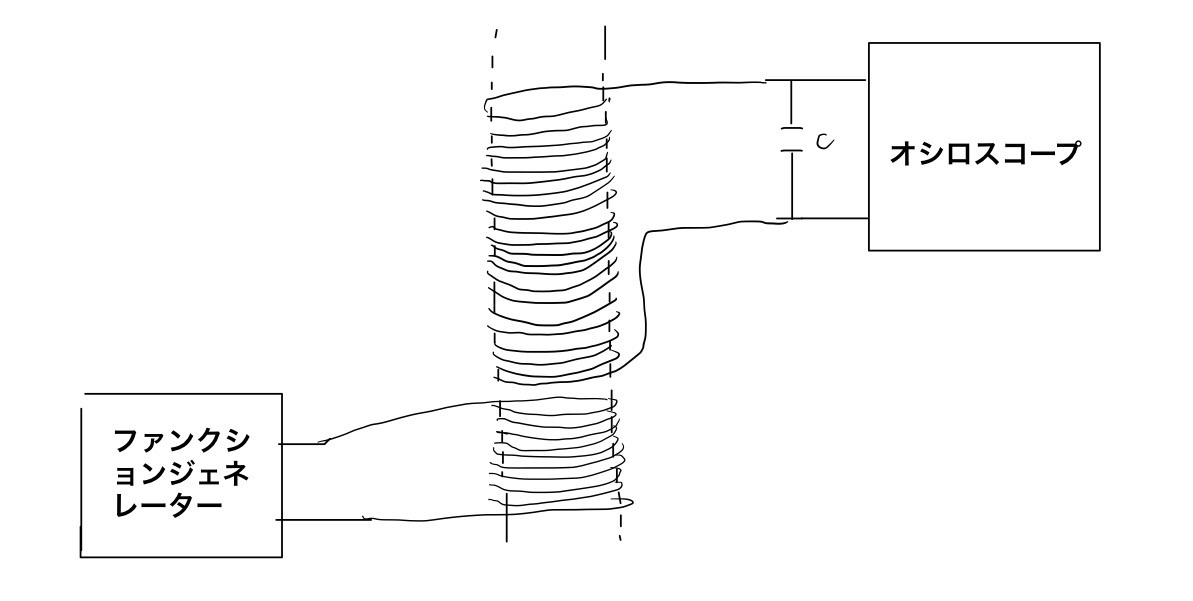
\includegraphics[height=5cm,clip]{kadono/image/houhou2.jpg}
\label{fig:ele1}
\caption{コイルの電磁誘導を使用したLC共鳴回路の模式図}
\end{figure}







\newpage
 \section{実験結果}
コンデンサの電気容量はLCRメータを用いて測定した値である。具体的なデータの値は付録を参照\\
電気容量45.8 pFの時の周波数と振幅の値の関係のグラフを次に示す。
\begin{figure}[H]
\centering
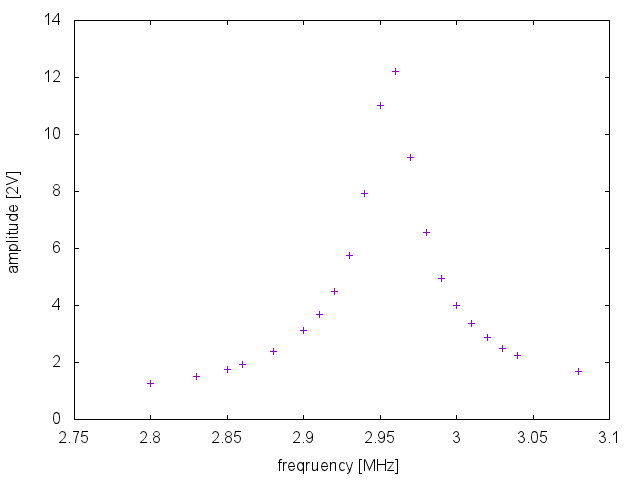
\includegraphics[height=7cm,clip]{kadono/image/45_8.png}
\label{fig:45.8}
\caption{45.8pFでの振動数[MHz]と振幅[V]の共鳴曲線}
\end{figure}
このときの共鳴振動数とその時の振幅$V_m$をグラフから読むと
\[
f_0=2.96\ {\rm MHz}\ \ \ V_m = 6.1\ {\rm V}
\]
であり、そのとき$V_m/\sqrt{2}$の値をとる振動数$f_1,f_2$は、データより
\[
f_1\sim 2.94\ {\rm MHz}\ \ \ f_2 \sim 2.975\ {\rm MHz}
\]
なので共鳴の鋭さQ値は
\[
Q=\frac{f_0}{f_2-f_1}\sim84.5
\]
となる。

他の電気容量の場合も45.8 pFの時と同様にして$f_0 , V_m , f_1 , f_2 , Q$を求める。その値を次の表に示す。各電気容量での振動数と振幅の関係のグラフは付録を参照
\begin{table}[H]
\caption{各電気容量の共鳴曲線から読み取れる値}
\centering
\begin{tabular}{c|c|c|c|c|c}
電気容量[pF]	&固有振動数$f_0$[MHz]	&最大振幅$V_m$[V]		&$f_1$[MHz]	&$f_2$[MHz]	&Q\\ \hline
45.8			&2.96					&6.1						&2.94		&2.975		&84.5\\
195.4		&1.49					&12.5					&1.44		&1.545		&14.2\\
292.0		&1.24					&12.4					&1.20		&1.285		&14.6\\
443.8		&1.00					&11.5					&0.97		&1.04		&14.3\\
663.0		&0.84					&17.7					&0.815		&0.855		&21.0\\\hline
\end{tabular}
\end{table}
上の表から電気容量が上がっていくにつれて共鳴振動数が減少していくことが分かる。この関係を図4に示す。\\
\begin{figure}[H]
\centering
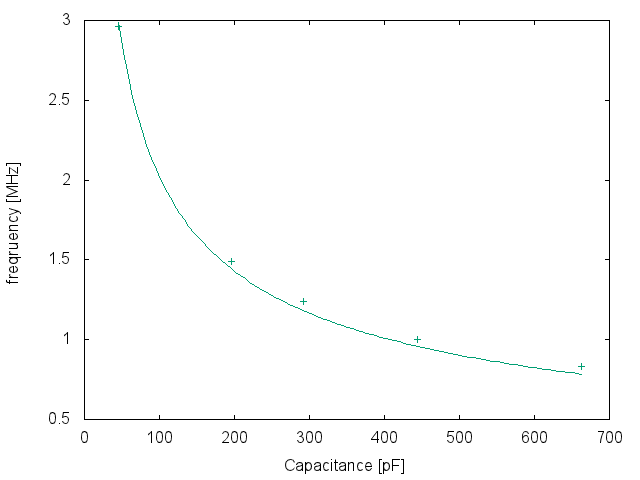
\includegraphics[height=8cm,clip]{kadono/image/all.png}
\label{fig:real}
\caption{共鳴振動数と電気容量の関係のグラフ}
\end{figure}
このグラフの線は各点が滑らかに引けると仮定して引いた線である。ここで理論によって導きだした式(3)と$f=\omega /2\pi$という関係より
\begin{eqnarray}
f_0=\frac{1}{2\pi \sqrt{LC}}
\end{eqnarray}
という関係式が導きだされる。この理論による数式と図4の曲線がどのくらい一致するか確認するために次に両対数のグラフを示した。
\begin{figure}[H]
\centering
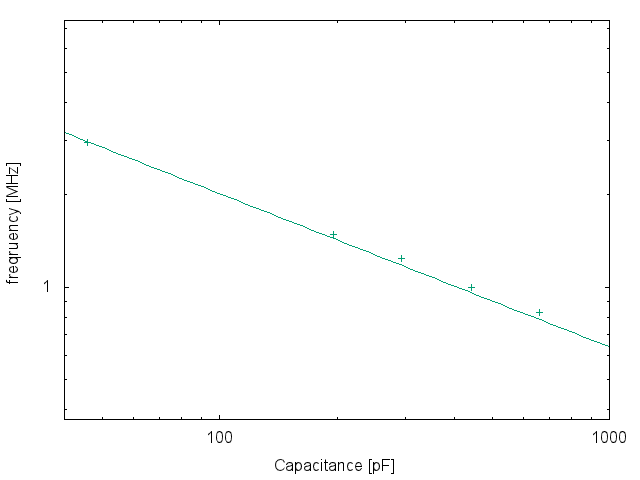
\includegraphics[height=8cm,clip]{kadono/image/f-clog.png}
\label{fig:logsc}
\caption{共鳴振動数と電気容量の関係の両対数グラフ}
\end{figure}
このグラフの線は各点のなるべく近くを通るように引いた線である。ここで最小二乗法を用いてこの線の傾きを求めると-0.48である。これはほとんど-1/2であるので共鳴振動数は電気容量の-1/2乗に比例することが確認された。\\
ここから自己インダクタンスLを求めることができることができるはずである。上記の共鳴振動数を求める数式(4)の両辺に対数をとると
\begin{eqnarray}
\log f_0= -\frac{1}{2}\log{C} + \log{\frac{1}{2 \pi \sqrt{L}}}
\end{eqnarray}
となる。ここで最小二乗法で求めた図5の切片は1.26であるので上の数式から今回作製したコイルの自己インダクタンスを求めると
\begin{eqnarray}
L=7.54 \times 10^{-5} {\rm H}
\end{eqnarray}
となる。







 \section{考察}
求めたQ値について評価すると、Qの値は電気容量が上がっていっても一定の変化をしているようには表1からは読み取れない。Q値が最大の値をとっている45.8pFの時の共鳴曲線と最小の値をとっている195.4pFの共鳴曲線を見比べてみると共鳴振動数の周辺での勾配が45.8pFの時のほうが大きくなっている。序論で言った通りQ値の値は共鳴の鋭さでありどれだけ効率よくエネルギーを吸収しているのかを示している値である。よって今回の実験の結果から45.8pFの時には安定してエネルギーが吸収されたことが分かる。しかし、45.8pFの以外の電気容量でのQ値はほとんど値が同じくらいである。Q値は
\[
Q=\frac{\omega_0}{\Delta \omega}=\frac{1}{\omega_0 RC}
\]
とも書き表せる。[3]この式から電気容量が増加するとQ値は減少するはずである。この結果は今回の実験と反している。今回の実験では45.8pFの時を測定して間を空けてほかの場合を測定してしていてその時にいろんな条件が変化してしまい何かノイズが生じてしまい振幅の値を誤って測定してしまった可能性がある。


次に今回の実験で求めた自己インダクタンスの値について別の視点から求めその値とどのくらい一致するのかを考察する。コイルの巻き数N, 断面積S, 長さlの自己インダクタンスは
\begin{eqnarray}
L=\frac{\mu_0 N^2 S}{l}
\end{eqnarray}
という関係式で求めることができる($\mu_0$は真空の透磁率)。[4] この関係を用いて今回使用したコイルのインダクタンスを求めると
\begin{eqnarray}
L = \frac{90^2 \times 10.5^2 \times \pi \times 10^{-3}\times \mu_0 }{0.4 \times 90 \times 10^{-3}}= 9.8 \times 10^{-5}\ \ [{\rm H}]
\end{eqnarray}
となる。ここで計算したコイルのインダクタンスの値は隙間ないく巻いているという条件で計算したものである、しかし今回作製したコイルはかなり簡易的なものでありところどころ隙間が目視できる状態であった。この点を考慮して(6)と(8)の値を比較するとほとんど同じような値であることが分かる。よって今回作成したコイルの自己インダクタンスは(6)の値であることが確認された。













 \section{結論}
今回使用したコイルの自己インダクタンスは$7.54\times10^{-5}$[H]であることが分かった。

\section*{参考文献}
\begin{enumerate}
  \item	兵頭俊夫著 考える力学 学術図書出版社
  \item 小形正男著 振動・波動 裳華房
  \item 宇田川眞行他編  物理学基礎実験 (第2版新訂) 共立出版株式会社 2012.
  \item 佐川弘幸・本間道雄著 物理学スーパーラーニングシリーズ 電磁気学 丸善出版 1997
  \item 小形正男著 振動・波動 (第11版) 裳華房 2008
\end{enumerate}

\section*{A付録 共鳴曲線}

\begin{figure}[H]
\centering
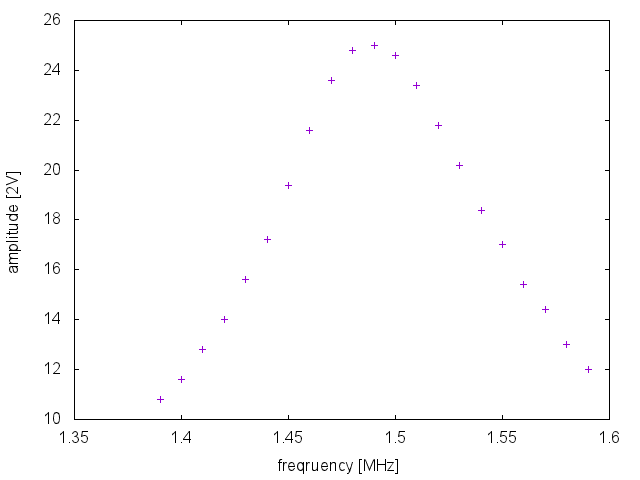
\includegraphics[height=5cm,clip]{kadono/image/195.png}
\label{fig:195.4}
\caption{195.4pFでの振動数[MHz]と振幅[V]の共鳴曲線}
\end{figure}
\begin{figure}[H]
\centering
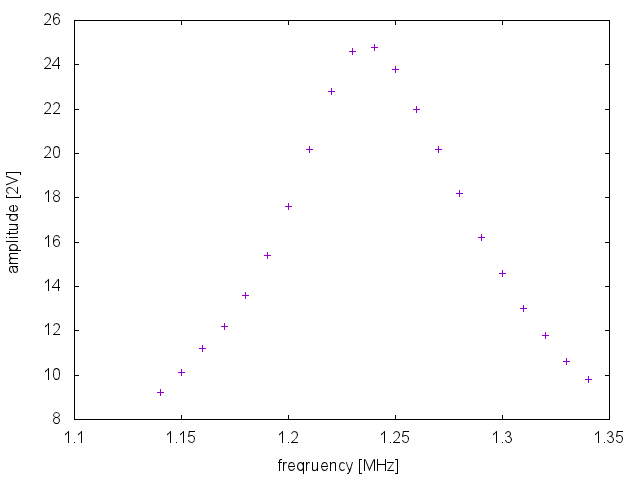
\includegraphics[height=5cm,clip]{kadono/image/292.png}
\label{fig:292.0}
\caption{292.0pFでの振動数[MHz]と振幅[V]の共鳴曲線}
\end{figure}
\begin{figure}[H]
\centering
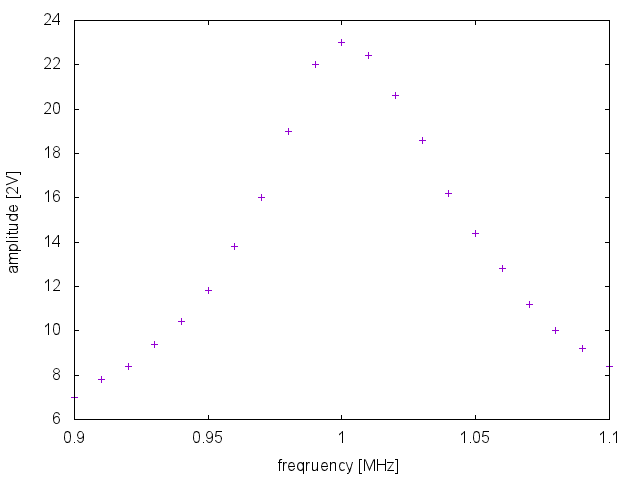
\includegraphics[height=5cm,clip]{kadono/image/443.png}
\label{fig:443.8}
\caption{443.8pFでの振動数[MHz]と振幅[V]の共鳴曲線}
\end{figure}
\begin{figure}[H]
\centering
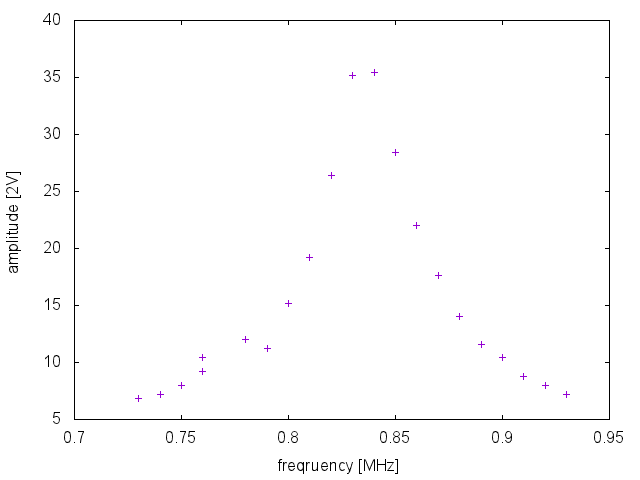
\includegraphics[height=5cm,clip]{kadono/image/663.png}
\label{fig:663}
\caption{663.0pFでの振動数[MHz]と振幅[V]の共鳴曲線}
\end{figure}
